\documentclass[tikz, border=15pt]{standalone}
\usetikzlibrary{positioning, arrows.meta}

\usepackage[T1]{fontenc}
\usepackage[utf8]{inputenc}
\usepackage{textcomp}
\renewcommand{\ttdefault}{lmtt}

\begin{document}
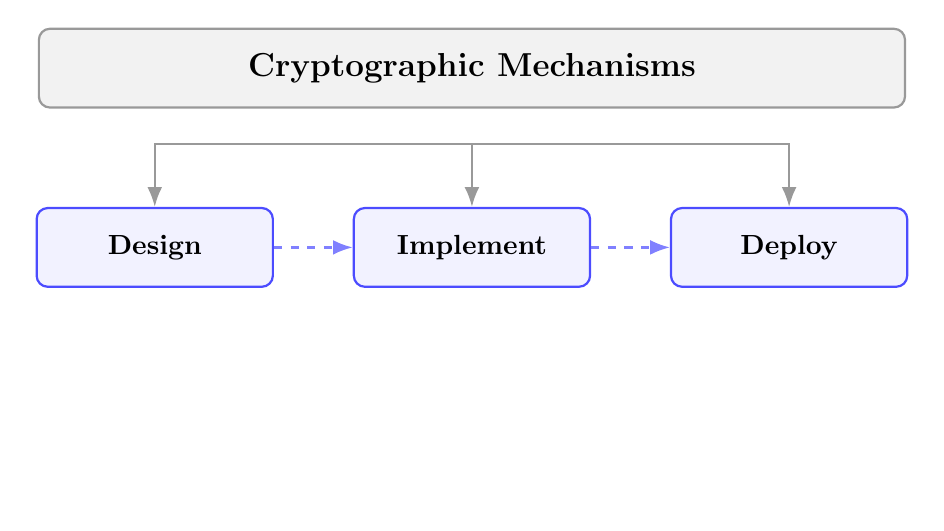
\begin{tikzpicture}[
	>=stealth,
	font=\sffamily,
	% Define styles
	titlebox/.style={rectangle, draw=gray!80, fill=gray!10, rounded corners, thick, minimum width=11cm, minimum height=1cm, font=\large\bfseries},
	phase/.style={rectangle, draw=blue!70, fill=blue!5, rounded corners, thick, minimum width=3cm, minimum height=1cm, font=\bfseries},
	failure/.style={rectangle, draw=white, fill=white, thick, dashed, minimum width=3.2cm, minimum height=1.2cm, align=center},
	arrow/.style={-{Latex[length=2.5mm]}, thick, gray!80},
	dangerarrow/.style={-{Latex[length=2.5mm]}, thick, red!70}
	]
	
	% 1. Main Subject
	\node[titlebox] (main) {Cryptographic Mechanisms};
	
	% Subtext
	\node[below=0.2cm of main, font=\small\color{gray!80!black}] (subtitle) {
%		Are difficult to \textbf{correctly}
	};
	
	% 2. Lifecycle Phases
	\node[phase, below=0.8cm of subtitle] (implement) {Implement};
	\node[phase, left=1cm of implement] (design) {Design};
	\node[phase, right=1cm of implement] (deploy) {Deploy};
	
	% Structural arrows for lifecycle connecting from the top
	\draw[arrow] (subtitle.south) -| (design.north);
	\draw[arrow] (subtitle.south) -- (implement.north);
	\draw[arrow] (subtitle.south) -| (deploy.north);
	
	% Process flow arrows between phases
	\draw[arrow, blue!50, dashed] (design) -- (implement);
	\draw[arrow, blue!50, dashed] (implement) -- (deploy);
	
	{\color{white}
	% 3. Failure Modes
	\node[failure, below=1.5cm of design] (flaws) {Flawed Security\\Arguments};
	\node[failure, below=1.5cm of implement] (bugs) {Implementation\\Bugs};
	\node[failure, below=1.5cm of deploy] (leakage) {Side-Channel\\Leakage};
	
%	% 4. Failure arrows
%	\draw[dangerarrow] (design.south) -- (flaws.north) node[midway, right, font=\scriptsize\color{red!70}, align=left] {Can fail\\due to};
%	\draw[dangerarrow] (implement.south) -- (bugs.north) node[midway, right, font=\scriptsize\color{red!70}, align=left] {Can fail\\due to};
%	\draw[dangerarrow] (deploy.south) -- (leakage.north) node[midway, right, font=\scriptsize\color{red!70}, align=left] {Can fail\\due to};
	
	% Optional: Cross-link for side channels (since they often manifest from implementation as well)
%	\draw[dangerarrow, opacity=0.4] (implement.south east) -- (leakage.north west);
	}
\end{tikzpicture}
\end{document}